\documentclass[tikz,border=10pt]{standalone}
\usepackage{tikz}
\usepackage{pgfplots}
\usepackage{amsmath}
\usetikzlibrary{shapes,arrows,positioning,calc,patterns,decorations.pathreplacing,backgrounds,fit,shadows}
\pgfplotsset{compat=1.16}

\begin{document}

% ========================================
% Figure 1: MVPP_MGC_PSO Overall Architecture
% ========================================
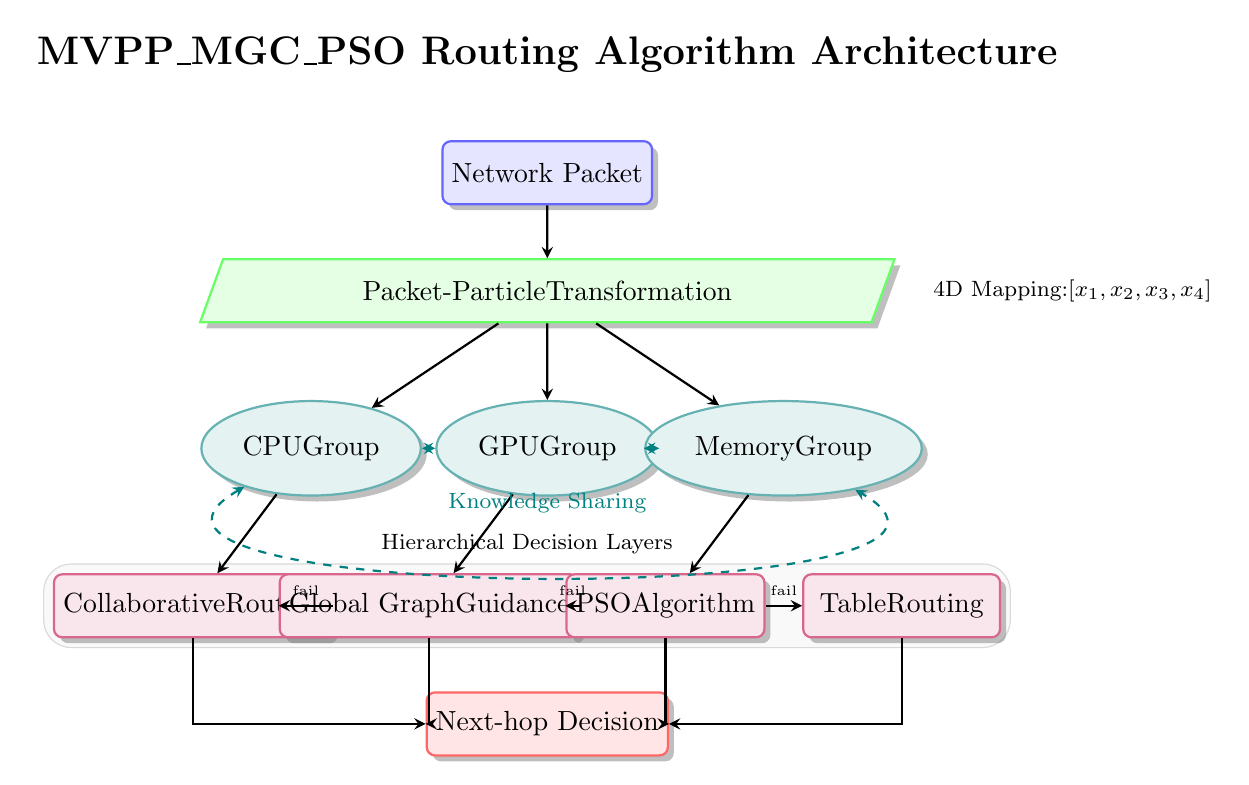
\begin{tikzpicture}[
    node distance=1.2cm and 1.5cm,
    % Style definitions
    packet/.style={rectangle, draw=blue!60, fill=blue!10, thick, minimum width=2cm, minimum height=0.8cm, rounded corners=3pt, drop shadow},
    transform/.style={trapezium, draw=green!60, fill=green!10, thick, minimum width=2.5cm, minimum height=0.8cm, trapezium left angle=70, trapezium right angle=110, drop shadow},
    decision/.style={diamond, draw=orange!60, fill=orange!10, thick, minimum width=2cm, minimum height=1cm, aspect=2, drop shadow},
    process/.style={rectangle, draw=purple!60, fill=purple!10, thick, minimum width=2.5cm, minimum height=0.8cm, rounded corners=3pt, drop shadow},
    output/.style={rectangle, draw=red!60, fill=red!10, thick, minimum width=2cm, minimum height=0.8cm, rounded corners=3pt, drop shadow},
    group/.style={ellipse, draw=teal!60, fill=teal!10, thick, minimum width=2.5cm, minimum height=1.2cm, drop shadow},
    arrow/.style={->, >=stealth, thick},
    doublearrow/.style={<->, >=stealth, thick}
]

% Title
\node[font=\Large\bfseries] at (0, 8) {MVPP\_MGC\_PSO Routing Algorithm Architecture};

% Layer 1: Input Processing
\node[packet] (input) at (0, 6.5) {Network Packet};
\node[transform] (particle) at (0, 5) {Packet-Particle\\Transformation};
\node[font=\footnotesize, right=0.5cm of particle] {4D Mapping:\\$[x_1, x_2, x_3, x_4]$};

% Layer 2: Multi-Group Clustering
\node[group] (cpu_group) at (-3, 3) {CPU\\Group};
\node[group] (gpu_group) at (0, 3) {GPU\\Group};
\node[group] (mem_group) at (3, 3) {Memory\\Group};

% Layer 3: Hierarchical Decision Framework
\node[process] (collab) at (-4.5, 1) {Collaborative\\Routing};
\node[process] (global) at (-1.5, 1) {Global Graph\\Guidance};
\node[process] (pso) at (1.5, 1) {PSO\\Algorithm};
\node[process] (table) at (4.5, 1) {Table\\Routing};

% Layer 4: Output
\node[output] (output) at (0, -0.5) {Next-hop Decision};

% Connections
\draw[arrow] (input) -- (particle);
\draw[arrow] (particle) -- (cpu_group);
\draw[arrow] (particle) -- (gpu_group);
\draw[arrow] (particle) -- (mem_group);

\draw[arrow] (cpu_group) -- (collab);
\draw[arrow] (gpu_group) -- (global);
\draw[arrow] (mem_group) -- (pso);

\draw[arrow] (collab) -- node[above, font=\tiny] {fail} (global);
\draw[arrow] (global) -- node[above, font=\tiny] {fail} (pso);
\draw[arrow] (pso) -- node[above, font=\tiny] {fail} (table);

\draw[arrow] (collab) |- (output);
\draw[arrow] (global) |- (output);
\draw[arrow] (pso) |- (output);
\draw[arrow] (table) |- (output);

% Inter-group collaboration arrows
\draw[doublearrow, dashed, teal] (cpu_group) -- (gpu_group);
\draw[doublearrow, dashed, teal] (gpu_group) -- (mem_group);
\draw[doublearrow, dashed, teal] (cpu_group) to[out=210,in=330] (mem_group);

% Annotations
\node[font=\footnotesize, text=teal] at (0, 2.3) {Knowledge Sharing};

% Background layers
\begin{scope}[on background layer]
    \node[draw=gray!30, fill=gray!5, rounded corners=10pt, fit=(collab)(table), label=above:{\footnotesize Hierarchical Decision Layers}] {};
\end{scope}

\end{tikzpicture}

% ========================================
% Figure 2: Packet-Particle Duality Concept
% ========================================
\begin{tikzpicture}[scale=0.9]

\node[font=\Large\bfseries] at (0, 7) {Packet-Particle Duality Transformation};

% Left side: Traditional Packet
\node[draw, rectangle, fill=blue!20, minimum width=3cm, minimum height=2cm] (packet) at (-4, 3) {
    \begin{tabular}{l}
        \textbf{Network Packet}\\
        \hline
        Source: Node 5\\
        Dest: Node 12\\
        Type: GPU\_SM\\
        Priority: High\\
        Size: 64 bytes
    \end{tabular}
};

% Transformation arrow
\draw[->, ultra thick, orange] (-2, 3) -- node[above] {$\phi$ Transformation} (2, 3);

% Right side: Particle in 4D space
\node[draw, rectangle, fill=green!20, minimum width=3.5cm, minimum height=2cm] (particle) at (4, 3) {
    \begin{tabular}{l}
        \textbf{PacketParticle}\\
        \hline
        Position: $[0.3, 0.8, 0.2, 0.9]$\\
        Velocity: $[0.1, -0.2, 0.3, 0.1]$\\
        $p_{best}$: $[0.2, 0.7, 0.3, 0.8]$\\
        Fitness: 0.342
    \end{tabular}
};

% 4D Space Visualization
\node at (0, 0) {
    \begin{tikzpicture}[scale=0.8]
        % Axes
        \draw[->] (0,0,0) -- (3,0,0) node[right] {$x_1$: Path Pref};
        \draw[->] (0,0,0) -- (0,3,0) node[above] {$x_2$: Load Bal};
        \draw[->] (0,0,0) -- (0,0,3) node[below left] {$x_3$: Power};
        \draw[dashed, ->] (0,0,0) -- (1.5,1.5,0) node[right] {$x_4$: Delay};
        
        % Particle position
        \fill[red] (0.9,2.4,0.6) circle (3pt);
        \node[font=\footnotesize] at (0.9,2.4,0.6) [above right] {Particle};
        
        % Velocity vector
        \draw[->, thick, blue] (0.9,2.4,0.6) -- (1.2,1.8,1.5);
    \end{tikzpicture}
};

\node[font=\footnotesize] at (0, -2) {4D Continuous Optimization Space};

\end{tikzpicture}

% ========================================
% Figure 3: Multi-Group Clustering Mechanism
% ========================================
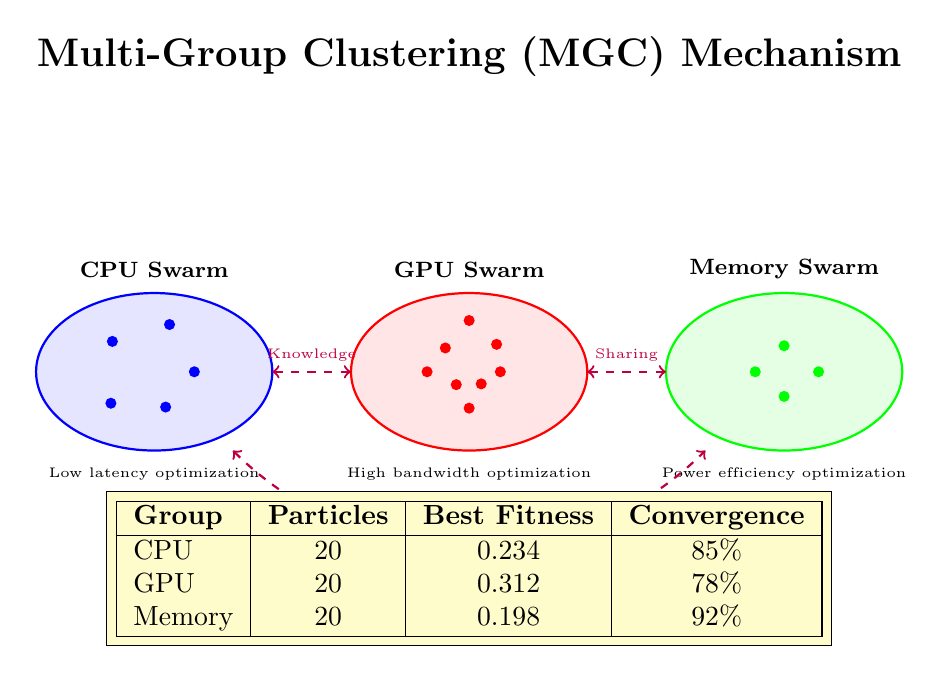
\begin{tikzpicture}

\node[font=\Large\bfseries] at (0, 6) {Multi-Group Clustering (MGC) Mechanism};

% Define swarm groups with particles
\begin{scope}[shift={(-4, 2)}]
    \draw[thick, blue, fill=blue!10] (0,0) ellipse (1.5cm and 1cm);
    \node[font=\footnotesize\bfseries] at (0, 1.3) {CPU Swarm};
    % Particles
    \foreach \i in {1,...,5} {
        \pgfmathsetmacro\angle{72*\i}
        \pgfmathsetmacro\radius{0.5+0.3*rand}
        \fill[blue] (\angle:\radius) circle (2pt);
    }
    \node[font=\tiny] at (0, -1.3) {Low latency optimization};
\end{scope}

\begin{scope}[shift={(0, 2)}]
    \draw[thick, red, fill=red!10] (0,0) ellipse (1.5cm and 1cm);
    \node[font=\footnotesize\bfseries] at (0, 1.3) {GPU Swarm};
    % Particles
    \foreach \i in {1,...,8} {
        \pgfmathsetmacro\angle{45*\i}
        \pgfmathsetmacro\radius{0.5+0.3*rand}
        \fill[red] (\angle:\radius) circle (2pt);
    }
    \node[font=\tiny] at (0, -1.3) {High bandwidth optimization};
\end{scope}

\begin{scope}[shift={(4, 2)}]
    \draw[thick, green, fill=green!10] (0,0) ellipse (1.5cm and 1cm);
    \node[font=\footnotesize\bfseries] at (0, 1.3) {Memory Swarm};
    % Particles
    \foreach \i in {1,...,4} {
        \pgfmathsetmacro\angle{90*\i}
        \pgfmathsetmacro\radius{0.5+0.3*rand}
        \fill[green] (\angle:\radius) circle (2pt);
    }
    \node[font=\tiny] at (0, -1.3) {Power efficiency optimization};
\end{scope}

% Inter-swarm collaboration
\draw[<->, thick, purple, dashed] (-2.5, 2) -- node[above, font=\tiny] {Knowledge} (-1.5, 2);
\draw[<->, thick, purple, dashed] (1.5, 2) -- node[above, font=\tiny] {Sharing} (2.5, 2);
\draw[<->, thick, purple, dashed] (-3, 1) to[out=-45,in=225] node[below, font=\tiny] {Migration} (3, 1);

% Performance metrics
\node[draw, fill=yellow!20] at (0, -0.5) {
    \begin{tabular}{|l|c|c|c|}
        \hline
        \textbf{Group} & \textbf{Particles} & \textbf{Best Fitness} & \textbf{Convergence}\\
        \hline
        CPU & 20 & 0.234 & 85\%\\
        GPU & 20 & 0.312 & 78\%\\
        Memory & 20 & 0.198 & 92\%\\
        \hline
    \end{tabular}
};

\end{tikzpicture}

% ========================================
% Figure 4: Hierarchical Decision Process
% ========================================
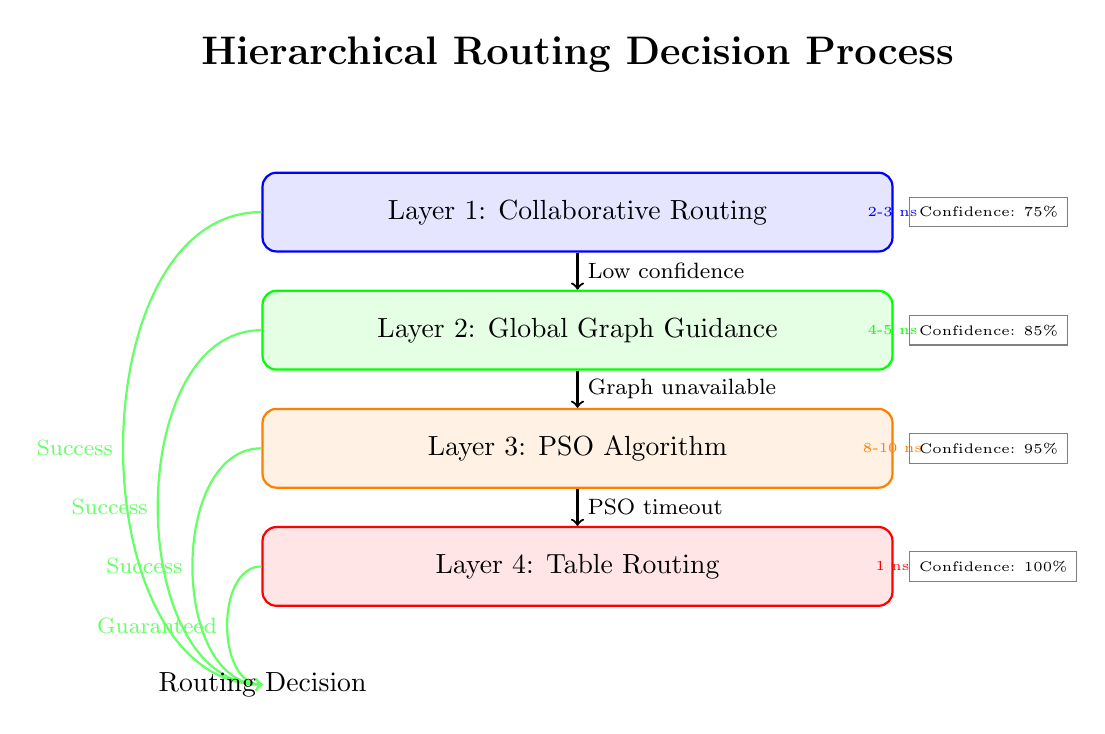
\begin{tikzpicture}[
    layer/.style={rectangle, draw=#1, fill=#1!10, thick, minimum width=8cm, minimum height=1cm, rounded corners=5pt},
    confidence/.style={rectangle, draw=gray, fill=white, font=\tiny}
]

\node[font=\Large\bfseries] at (0, 7) {Hierarchical Routing Decision Process};

% Layers
\node[layer=blue] (l1) at (0, 5) {Layer 1: Collaborative Routing};
\node[confidence, right=0.2cm of l1] {Confidence: 75\%};

\node[layer=green] (l2) at (0, 3.5) {Layer 2: Global Graph Guidance};
\node[confidence, right=0.2cm of l2] {Confidence: 85\%};

\node[layer=orange] (l3) at (0, 2) {Layer 3: PSO Algorithm};
\node[confidence, right=0.2cm of l3] {Confidence: 95\%};

\node[layer=red] (l4) at (0, 0.5) {Layer 4: Table Routing};
\node[confidence, right=0.2cm of l4] {Confidence: 100\%};

% Decision flow
\draw[->, thick] (l1) -- node[right, font=\footnotesize] {Low confidence} (l2);
\draw[->, thick] (l2) -- node[right, font=\footnotesize] {Graph unavailable} (l3);
\draw[->, thick] (l3) -- node[right, font=\footnotesize] {PSO timeout} (l4);

% Success paths
\draw[->, thick, green!60] (l1.west) to[out=180,in=180] node[left, font=\footnotesize] {Success} (-4, -1);
\draw[->, thick, green!60] (l2.west) to[out=180,in=180] node[left, font=\footnotesize] {Success} (-4, -1);
\draw[->, thick, green!60] (l3.west) to[out=180,in=180] node[left, font=\footnotesize] {Success} (-4, -1);
\draw[->, thick, green!60] (l4.west) to[out=180,in=180] node[left, font=\footnotesize] {Guaranteed} (-4, -1);

\node[output/.style] at (-4, -1) {Routing Decision};

% Timing annotations
\node[font=\tiny, text=blue] at (4, 5) {2-3 ns};
\node[font=\tiny, text=green] at (4, 3.5) {4-5 ns};
\node[font=\tiny, text=orange] at (4, 2) {8-10 ns};
\node[font=\tiny, text=red] at (4, 0.5) {1 ns};

\end{tikzpicture}

% ========================================
% Figure 5: Performance Comparison Charts
% ========================================
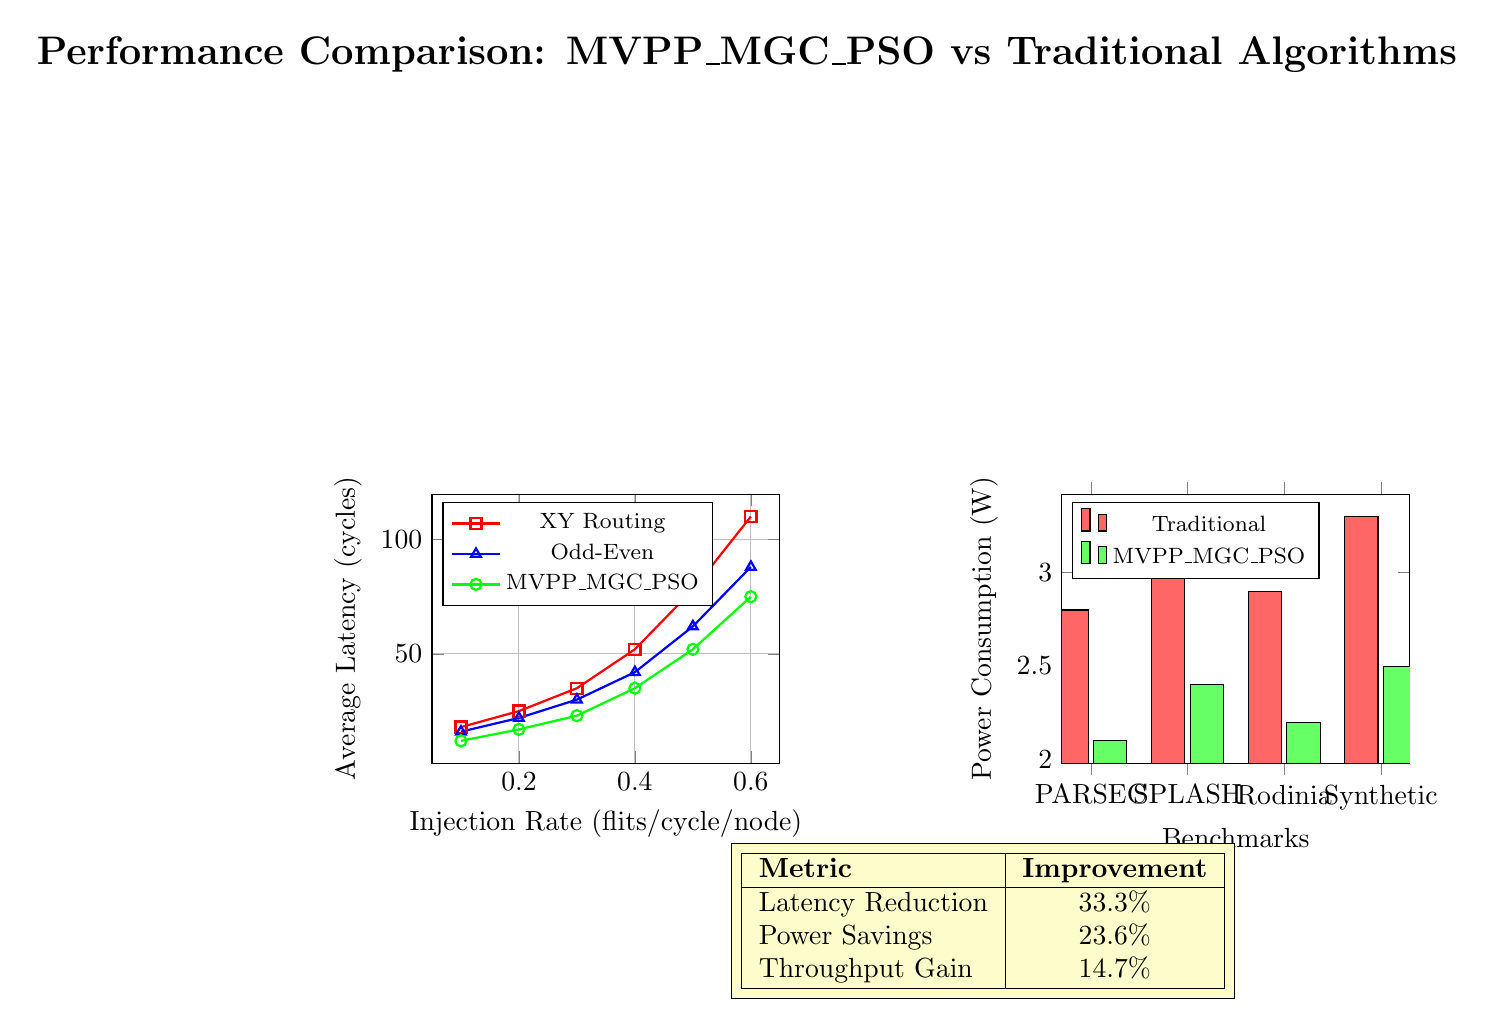
\begin{tikzpicture}

\node[font=\Large\bfseries] at (4, 9) {Performance Comparison: MVPP\_MGC\_PSO vs Traditional Algorithms};

% Latency comparison
\begin{axis}[
    at={(0,0)},
    width=6cm,
    height=5cm,
    xlabel={Injection Rate (flits/cycle/node)},
    ylabel={Average Latency (cycles)},
    legend pos=north west,
    grid=major,
    legend style={font=\footnotesize}
]
\addplot[color=red, mark=square, thick] coordinates {
    (0.1, 18) (0.2, 25) (0.3, 35) (0.4, 52) (0.5, 78) (0.6, 110)
};
\addlegendentry{XY Routing}

\addplot[color=blue, mark=triangle, thick] coordinates {
    (0.1, 16) (0.2, 22) (0.3, 30) (0.4, 42) (0.5, 62) (0.6, 88)
};
\addlegendentry{Odd-Even}

\addplot[color=green, mark=o, thick] coordinates {
    (0.1, 12) (0.2, 17) (0.3, 23) (0.4, 35) (0.5, 52) (0.6, 75)
};
\addlegendentry{MVPP\_MGC\_PSO}
\end{axis}

% Power consumption comparison
\begin{axis}[
    at={(8cm,0)},
    width=6cm,
    height=5cm,
    ybar,
    bar width=12pt,
    xlabel={Benchmarks},
    ylabel={Power Consumption (W)},
    symbolic x coords={PARSEC, SPLASH, Rodinia, Synthetic},
    xtick=data,
    legend pos=north west,
    legend style={font=\footnotesize}
]
\addplot[fill=red!60] coordinates {
    (PARSEC, 2.8) (SPLASH, 3.1) (Rodinia, 2.9) (Synthetic, 3.3)
};
\addlegendentry{Traditional}

\addplot[fill=green!60] coordinates {
    (PARSEC, 2.1) (SPLASH, 2.4) (Rodinia, 2.2) (Synthetic, 2.5)
};
\addlegendentry{MVPP\_MGC\_PSO}
\end{axis}

% Improvement metrics
\node[draw, fill=yellow!20] at (7, -2) {
    \begin{tabular}{|l|c|}
        \hline
        \textbf{Metric} & \textbf{Improvement}\\
        \hline
        Latency Reduction & 33.3\%\\
        Power Savings & 23.6\%\\
        Throughput Gain & 14.7\%\\
        \hline
    \end{tabular}
};

\end{tikzpicture}

% ========================================
% Figure 6: PSO Convergence Behavior
% ========================================
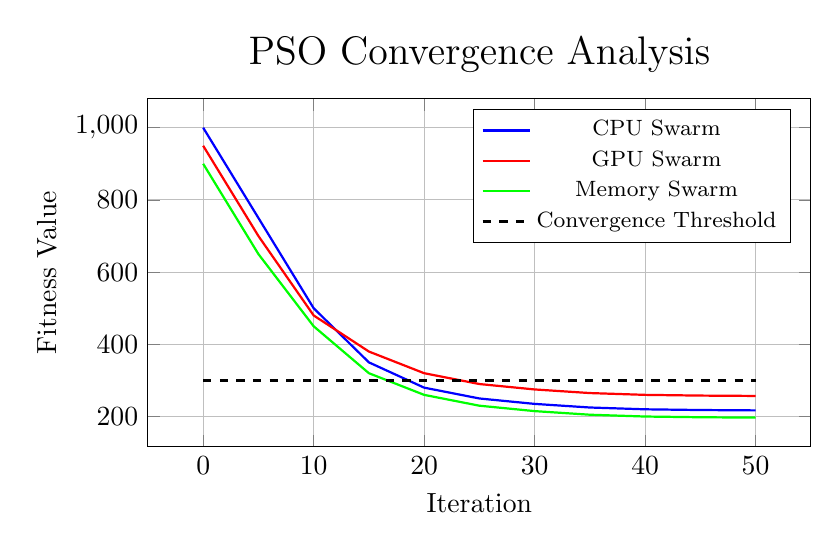
\begin{tikzpicture}

\begin{axis}[
    width=10cm,
    height=6cm,
    xlabel={Iteration},
    ylabel={Fitness Value},
    title={\Large PSO Convergence Analysis},
    legend pos=north east,
    grid=major,
    legend style={font=\footnotesize}
]

% CPU Swarm
\addplot[color=blue, thick, mark=none] coordinates {
    (0, 1000) (5, 750) (10, 500) (15, 350) (20, 280) (25, 250) 
    (30, 235) (35, 225) (40, 220) (45, 218) (50, 217)
};
\addlegendentry{CPU Swarm}

% GPU Swarm
\addplot[color=red, thick, mark=none] coordinates {
    (0, 950) (5, 700) (10, 480) (15, 380) (20, 320) (25, 290) 
    (30, 275) (35, 265) (40, 260) (45, 258) (50, 257)
};
\addlegendentry{GPU Swarm}

% Memory Swarm
\addplot[color=green, thick, mark=none] coordinates {
    (0, 900) (5, 650) (10, 450) (15, 320) (20, 260) (25, 230) 
    (30, 215) (35, 205) (40, 200) (45, 198) (50, 197)
};
\addlegendentry{Memory Swarm}

% Convergence threshold
\addplot[color=black, dashed, thick] coordinates {
    (0, 300) (50, 300)
};
\addlegendentry{Convergence Threshold}

\end{axis}

\end{tikzpicture}

% ========================================
% Figure 7: Multi-Objective Optimization Radar Chart
% ========================================
\begin{tikzpicture}[scale=1.2]

\node[font=\Large\bfseries] at (0, 5) {Multi-Objective Optimization Performance};

% Radar chart axes
\def\numvars{6}
\def\radius{3}

% Draw axes
\foreach \i in {1,...,\numvars} {
    \pgfmathsetmacro\angle{90 - (\i-1)*360/\numvars}
    \draw[thick] (0,0) -- (\angle:\radius);
}

% Draw grid
\foreach \r in {0.6,1.2,1.8,2.4,3} {
    \draw[gray, dashed] (90:\r) 
        \foreach \i in {2,...,\numvars} {
            \pgfmathsetmacro\angle{90 - (\i-1)*360/\numvars}
            -- (\angle:\r)
        } -- cycle;
}

% Labels
\node[above] at (90:3.2) {Latency};
\node[above right] at (30:3.2) {Power};
\node[below right] at (-30:3.2) {Reliability};
\node[below] at (-90:3.2) {Load Balance};
\node[below left] at (-150:3.2) {Congestion};
\node[above left] at (150:3.2) {QoS};

% Traditional routing (red)
\draw[thick, red, fill=red!20, opacity=0.5] 
    (90:1.8) -- (30:1.5) -- (-30:1.2) -- (-90:1.3) -- (-150:1.4) -- (150:1.6) -- cycle;

% MVPP_MGC_PSO (green)
\draw[thick, green, fill=green!20, opacity=0.5] 
    (90:2.7) -- (30:2.5) -- (-30:2.6) -- (-90:2.8) -- (-150:2.7) -- (150:2.6) -- cycle;

% Legend
\node[draw, fill=red!20] at (-4, -1) {Traditional};
\node[draw, fill=green!20] at (-4, -1.7) {MVPP\_MGC\_PSO};

\end{tikzpicture}

\end{document}